\documentclass[a4paper,11pt,answers,11pt]{exam}
\usepackage{enumerate}
\usepackage{wrapfig}
\usepackage{fullpage}
\usepackage{textcomp}
\usepackage{charter}
\usepackage[utf8]{inputenc}
\usepackage[T1]{fontenc}
\usepackage[frenchb]{babel}
\usepackage{url}
\usepackage{graphicx} % insertion d'images 
\usepackage{hyperref}
\usepackage{lmodern}  % improve pdf rendering
\usepackage{listings} % coloration code
\usepackage{cite}
\usepackage{caption}
\usepackage{upquote}
\usepackage{xcolor}
\usepackage{color}
\usepackage{amssymb,amsmath}
\usepackage{algorithm}
\usepackage{algorithmic}
\usepackage{amsmath}
\bibliographystyle{unsrt}

\lstset{
	language=C,                     % choose the language of the code
	basicstyle=\footnotesize,       % the size of the fonts that are used for the code
	numbers=left,                   % where to put the line-numbers
	numberstyle=\footnotesize,      % the size of the fonts that are used for the line-numbers
	stepnumber=1,                   % the step between two line-numbers. If it is 1 each line will be numbered
	numbersep=5pt,                  % how far the line-numbers are from the code
	backgroundcolor=\color{white},  % choose the background color. You must add \usepackage{color}
	showspaces=false,               % show spaces adding particular underscores
	showstringspaces=false,         % underline spaces within strings
	showtabs=false,                 % show tabs within strings adding particular underscores
	frame=single,                   % adds a frame around the code
	tabsize=2,                      % sets default tabsize to 2 spaces
	captionpos=b,                   % sets the caption-position to bottom
	breaklines=true,                % sets automatic line breaking
	breakatwhitespace=false,        % sets if automatic breaks should only happen at whitespace
	escapeinside={\%*}{*)},         % if you want to add a comment within your code
	identifierstyle=\ttfamily,
	keywordstyle=\color[rgb]{0,0,1},
	commentstyle=\color[rgb]{0.133,0.545,0.133},
	stringstyle=\color[rgb]{0.627,0.126,0.941}
}

\renewcommand{\solutiontitle}{\noindent\textbf{Aide :}\par\noindent} % Définit le titre des solutions

\definecolor{darkred}{rgb}{0.5,0,0}
\definecolor{darkgreen}{rgb}{0,0.5,0}
\definecolor{darkblue}{rgb}{0,0,0.5}

\hypersetup{
	colorlinks=true,
	%linkcolor=red,%
	linkcolor=darkred,
	filecolor=darkred,
	urlcolor=darkblue,
	citecolor=darkgreen
}

\captionsetup{
  figurename={\sc Fig.},
  tablename={\sc Tab.}
}

% numérotation
\setcounter{tocdepth}{2}    % profondeur 
\setcounter{secnumdepth}{3} % profondeur

% Propriétés doc
\title{Problème à $N$ corps - Attraction gravitationnelle}
\author{Adrien Cassagne}
\date{14 mars 2014}

\begin{document}
\begin{title}
\noindent\makebox[\textwidth][c]{
	\noindent\makebox[\textwidth][c]{
		
\includegraphics[scale=0.25]{images/logo_cines_small.jpeg}
	}
}
\begin{center}
	{\Large{Problème à $N$ corps - Attraction gravitationnelle}}\\
\end{center}
\begin{center}
	{\footnotesize{Formation MPI/OpenMP - Adrien {\sc Cassagne}}}
\end{center}
\end{title}

\setcounter{page}{1}
\section {Introduction}
Le problème à $N$ corps (\textit{N-body} dans la littérature anglaise) est un problème assez classique de la mécanique de {\sc Newton}: il consiste en la résolution des équations du mouvement de {\sc Newton}. 
Ce problème peut cependant être généralisé et on le rencontre assez fréquemment dans la simulation numérique: cela fait de lui un bon cas d'école.

Au départ du problème (à l'instant $t$), pour chaque corps $i$, sa position $\vec{q_t}(i)$, sa masse $m_i$ et sa vitesse $\vec{v_t}(i)$ sont connues.
La force exercée entre deux corps $i$ et $j$, à un instant $t$ donné, est définie comme suit:
\begin{equation}
\label{eq:force}
	\vec{F_t}(i,j) = G.\frac{m_i.m_j}{(D_{i,j})^2}.\vec{u},
\end{equation}
avec $G$ la constante gravitationnelle ($G = 6,67384\times10^{-11} m^3.kg^{-1}.s^{-2}$), $D_{i,j}$ la distance entre un corps $i$ et un corps $j$ et $\vec{u}$ le vecteur unitaire dirigé de $i$ vers $j$.
La force résultante pour un corps $i$ donné, à un instant $t$ donné, est la suivante:
\begin{equation}
\label{eq:somForce}
	\vec{F_t}(i) = \sum_{j \ne i}^{N} \vec{F_t}(i,j),
\end{equation}
avec $N$ le nombre de corps présents dans l'espace.
L'accélération pour un corps $i$, à un instant $t$ donné, est la suivante:
\begin{equation}
\label{eq:acceleration}
	\vec{a_t}(i) = \frac{\vec{F_t}(i)}{m_i}.
\end{equation}
La vitesse d'un corps $i$ à un instant $t + dt$ dépend de la vistesse et de l'accélération à l'instant $t$:
\begin{equation}
\label{eq:vitesse}
	\vec{v_{t+dt}}(i) = \vec{v_{t}}(i) + \vec{a_t}(i).dt.
\end{equation}
Enfin, la position $q$ d'un corps $i$ à l'instant $t + dt$ dépend de la position, de la vitesse et de l'accélération à l'instant $t$:
\begin{equation}
\label{eq:position}
	\vec{q_{t+dt}}(i) = \vec{q_{t}}(i) + \vec{v_{t}}(i).dt + \frac{\vec{a_t}(i).dt^2}{2}.
\end{equation}
Grâce aux équations \ref{eq:force}, \ref{eq:somForce}, \ref{eq:acceleration}, \ref{eq:vitesse} et \ref{eq:position} il est possible de calculer la nouvelle position et la nouvelle vitesse pour tous corps $i$ à l'instant $t + dt$.

\subsection{Choix du pas de temps $dt$}
Le plus simple est de choisir un pas de temps constant entre toutes les itérations cependant cela ne permet pas d'observer finement les intéractions surtout quand les corps se rapprochent de plus en plus.
Nous avons donc fait le choix de calculer un nouveau pas de temps à chaque itération pour qu'il soit adapté à la simulation.
Par soucis de simplicité ce pas de temps $dt$ sera commun à tout les corps du plan et devra respecter la condition suivante:
\begin{equation}
\label{eq:dt1}
	\|\vec{v_t}(i).dt + \frac{\vec{a_t}(i)}{2}.dt^2 \| \leq 0.1\times D_{i,j},
\end{equation}
avec $j$ le corps le plus proche de $i$.
Pour chaque corps $i$, un pas de temps sera calculé et le plus petit de ces pas de temps sera choisi.
L'équation~\ref{eq:dt1} traduit que la distance entre $i_t$ et $i_{t+dt}$ doit être inférieure à 10\% de la distance entre $i_t$ et $j_t$.
Cela assure que deux masses quelconques ne se rapprochent pas plus de 20\% entre les instants $t$ et $t + dt$.
Cependant, l'équation~\ref{eq:dt1} n'est pas directement utilisable, elle donne lieu à la résolution d'un polynôme de degré 4 en $dt$.
C'est pour cela que nous utilisons l'inégalité triangulaire qui permet de déterminer une nouvelle condition:
\begin{equation}
\label{eq:dt2}
	\|\vec{v_t}(i)\|.dt + \frac{\|\vec{a_t}(i)\|}{2}.dt^2  \leq 0.1\times D_{i,j}.
\end{equation}
L'équation~\ref{eq:dt2} est de degré 2 ce qui est beaucoup plus raisonnable en de temps de calcul.

\subsection{Traduction algorithmique}
D'un point de vue algorithmique, on calcule chaque corps en fonction de tous les autres.
Cela se résume en l'imbrication de deux boucles \texttt{for} allant de $0$ à $N$ corps.
Dans un langage \texttt{C-like} on peut l'exprimer de la façon suivante:
\begin{lstlisting}[caption={Pseudo code illustrant un algorithme de type $N$ corps},label={alg:ncorps}]
body b1[N]; // array which contains all bodies (at t)
body b2[N]; // empty array
for(unsigned int iBody = 0; iBody < N; ++iBody)
	for(unsigned int jBody = 0; jBody < N; ++jBody)
		if(iBody != jBody)
			b2[iBody] = compute(b1[jBody]);
\end{lstlisting}
L'algorithme \ref{alg:ncorps} montre une propriété très importante de cette classe de problème: pour $N$ corps donnés, la complexité en terme de calcul est de $O(N^2)$. 
Il existe cependant une méthode permettant d'approximer et de résoudre le problème en $O(N \log{N} )$ mais nous ne l'utiliserons pas dans ce T.D. (voir simulation de {\sc Barnes-Hut}).
%Cela permet théoriquement de recouvrir les temps de communications MPI par du calcul.



\section {Objectifs}
Dans ce T.D. il est question d'utiliser les bases MPI et OpenMP acquises lors des précédents travaux et de les combiner sur un cas physique réel.
Plus précisément nous allons:
\begin{enumerate}
	\item simuler le déplacement de $N$ corps dans le plan,
	\item paralléliser les traitements d'un n\oe ud avec OpenMP,
	\item mettre en place un anneau de communication MPI,
	\item paralléliser les traitements multi-n\oe uds avec MPI,
	\item recouvrir les temps de communication par du calcul.
\end{enumerate}

Nous allons effectuer une simulation dans le plan car il est relativement simple de la visionner sur un écran.
Les corps seront répartis sur les processus MPI. Cela permet de traiter plus de corps que la limite mémoire d'un n\oe ud le permet.


\section {Préparation}
Afin de ne pas perdre de temps, nous partirons d'un code séquentiel fonctionnel dans lequel toute la physique a déjà été implémentée.
En premier lieu vous devez décompresser l'archive \textit{nbody.tar.gz} dans votre \textit{/home/\$USER}:
\texttt{tar -xvvf nbody.tar.gz}.
Vous possédez maintenant un dossier \textit{/home/\$USER/nbody/} contenant les fichiers/dossiers suivants:
\begin{itemize}
\item \textit{Makefile}: le \textit{Makefile} permettant de compiler le projet,
\item \textit{bin/}: dossier contenant les exécutables,
\item \textit{data/}: dossier contenant les cas de test,
\item \textit{doc/}: dossier contenant des documents relatifs au projet (comme ce sujet),
\item \textit{obj/}: dossier contenant les fichiers compilés avant l'édition de liens,
\item \textit{objd/}: dossier contenant les fichiers compilés avant l'édition de liens (en mode debug),
\item \textit{reader/}: fichier source du code de visualisation des résulats d'une simulation,
\item \textit{src/}: dossier contenant le code source.
\end{itemize}
Pour compiler le code dans sa version séquentielle il suffit de taper la commande \texttt{make} et l'exécutable se construit dans \textit{bin/nbody}.
Le code source est écrit en \texttt{C 99} qui permet un peu plus de souplesse que le \texttt{C} traditionnel.

\subsection{Les sources}

\subsubsection{Le point d'entrée: le \texttt{main}}
Le point d'entrée du programme (fonction \texttt{main}) est contenu dans \textit{src/main.c}.
C'est dans ce fichier que sont définies les trois grandes étapes autour de la boucle des itérations (cf. list.~\ref{alg:iterations}):
\begin{enumerate}
\item calculer l'accélération de tous les corps du plan \texttt{p},
\item rechercher le plus petit pas de temps \texttt{dt} et le choisir pour tous les corps,
\item mettre à jour la position et la vitesse de tous les corps du plan.
\end{enumerate}
\begin{lstlisting}[caption={Code simplifié du calcul par itération},label={alg:iterations}]
void main()
{
	double dt;
	plan *p = createPlan(); // p contains the bodies
	for(unsigned long iIte = 1; iIte <= NIterations; ++iIte) 
	{
		computeAllLocalAcceleration(p);
		dt = findLocalDt(p);
		updateAllLocalPositionAndSpeed(p, dt);
	}
}
\end{lstlisting}
Les structures utilisées (ici \texttt{plan}) sont détaillées dans les sections suivantes.

\subsubsection{Module \texttt{body}}
Le module \texttt{body} (fichiers \textit{src/body.c} et \textit{src/body.h}) contient la structure \texttt{body}:
\begin{lstlisting}[caption={Structure \texttt{body}},label={alg:strBody}]
typedef struct 
{
	double mass; // body mass
	double posX; // body position following x axis
	double posY; // body position following y axis
} body;
\end{lstlisting}
Ainsi que la structure \texttt{localBody}:
\begin{lstlisting}[caption={Structure \texttt{localBody}},label={alg:strLocalBody}]
typedef struct 
{
	body   *b;                 // body mass and body position
	double speedX;             // body speed following x axis
	double speedY;             // body speed following y axis
	double accelerationX;      // body acceleration following x axis
	double accelerationY;      // body acceleration following y axis
	double closestNeighborLen; // contains the distance with the closest neighbor
} localBody;
\end{lstlisting}
Nous avons choisi d'utiliser deux structures (\texttt{body} et \texttt{localBody}) afin de décrire complètement les propriétés d'un corps.
La structure \texttt{body} (cf. list.~\ref{alg:strBody}) contient la masse et la position du corps et la structure \texttt{localBody} (cf. list.~\ref{alg:strLocalBody}) ajoute la vitesse et l'accélération.
Cela est inutile pour le code séquentiel (on aurait pu mettre tous les champs dans une même structure) cependant quand vous implémenterez le code parallèle MPI, seules les propriétés de la structure \texttt{body} seront à communiquer aux autres n\oe uds.
Les données supplémentaires de \texttt{localBody} sont uniquement nécessaires pour le calcul local à un processus.

\subsubsection{Module \texttt{plan}}
Le module \texttt{plan} (fichiers \textit{src/plan.c} et \textit{src/plan.h}) contient la structure \texttt{plan}:
\begin{lstlisting}[caption={Structure \texttt{plan}},label={alg:strPlan}]
typedef struct
{
	unsigned long nBody; // bodies number
	localBody     *lb;   // local body array values
} plan;
\end{lstlisting}
Un plan (cf. list.~\ref{alg:strPlan}) contient le nombre de corps \texttt{nBody} ainsi que les propriétés de chacun de ces corps dans le tableau \texttt{lb} (masse, position, vitesse et accélération).

\subsubsection{Simuler un cas de test}
Après avoir compilé le code (commande \texttt{make}), vous pouvez essayer de lancer un cas de test en exécutant le code comme suit:
\begin{equation*}
\texttt{> ./bin/nbody -f data/in/in.testcase.1.dat -i 100 -v -w}
\end{equation*}
L'option \texttt{-f} permet de spécifier un fichier d'entrée, l'option \texttt{-i} permet de choisir le nombre d'itérations à calculer, l'option \texttt{-v} active le mode verbose et enfin l'option \texttt{-w} permet d'écrire la solution à chaque itération dans \textit{data/out/out.*.dat} (\textit{*} correspond au numéro de l'itération).

Pour visualiser les solutions il faut compiler le \texttt{reader} avec la commande \texttt{make reader} et pour l'exécuter vous pouvez utiliser la commande suivante:
\begin{equation*}
\texttt{> ./bin/reader 800 600 data/out/out}
\end{equation*}
Les deux premiers paramètres définissent la taille de la fenêtre de visualisation et le dernier paramètre permet de spécifier la racine des noms des fichiers à visualiser.
Un fois la fenêtre de visualisation ouverte, appuyez sur la touche "flêche droite" pour lancer l'animation.

Si vous voyez deux corps s'éloigner puis se rapprocher alors le code fonctionne correctement et vous pouvez passer aux exercices de la section suivante.


\section {Exercices}
\begin{questions}
	\question Paralléliser le code séquentiel initial avec OpenMP.
	\begin{solution}
		Avant de foncer tête baissée, il est bon de refléchir un peu et de trouver où l'on passe le plus de temps : c'est cette zone qu'il faut essayer de paralléliser.
		Ici, il n'est pas question d'utiliser des primitives très complexes, un simple \texttt{\#pragma omp parallel for schedule(runtime)} devrait suffir.
		Vous pourrez ensuite définir, à l'exécution du code, les variables d'environnement \texttt{OMP\_NUM\_THREADS} et \texttt{OMP\_SCHEDULE} afin de trouver le meilleur compromis pour les performances. 
	\end{solution}
	\question Créer une structure MPI (\texttt{MPI\_BODY}) pour envoyer/recevoir des corps.
	\begin{solution}
		La structure \texttt{body} qui est déclarée dans le fichier \textit{src/body.h} ne fait pas partie des types de base que connaît MPI.
		Il faut donc déclarer une nouvelle structure MPI suivant les spécifications de la structure \texttt{body}.
		La création de structure MPI est assurée par la routine \texttt{MPI\_Type\_struct}.
		Une fois la structure MPI créée il faut nécessairement la déclarer avec la routine \texttt{MPI\_Type\_commit}.
		Avant de quitter le programme il faut penser à libérer la mémoire utilisée par la structure en appelant \texttt{MPI\_Type\_free}.
	\end{solution}
	\question Mettre en place un anneau de communication MPI (voir fig.~\ref{fig:anneau}).
	\begin{figure}[htbp]
		\centering
		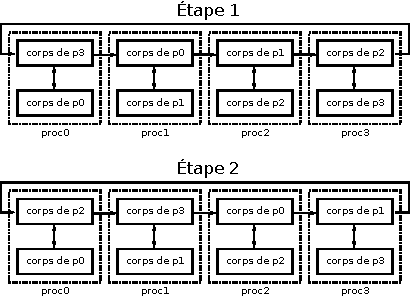
\includegraphics[width=0.6\linewidth]{schemas/anneau_sans_buffering.pdf}
		\caption{Anneau de communication pour 4 processus MPI}
		\label{fig:anneau}
	\end{figure}
	\begin{solution}
		Une itération est complète quand tous les processus MPI ont reçu les corps de tous les autres processus.
		Pour y parvenir il y a deux phases:
		\begin{itemize}
			\item l'initialisation: chaque processus envoie ses corps à son voisin de droite (et reçoit de son voisin de gauche),
			\item ensuite il faut simplement que chaque processus envoie le \textit{buffer} qu'il reçoit de son voisin de gauche à son voisin de droite.
		\end{itemize}
		Au final, il y a autant d'envoi et de réception qu'il y a de processus MPI.
		La réception et l'envoi peuvent être réalisés de façon bloquante avec les routines \texttt{MPI\_Recv} et \texttt{MPI\_Send}.
	\end{solution}
	\question Trouver le plus petit pas de temps $dt$ parmi tout les processus MPI et le choisir.
	\begin{solution}
		À chaque itération, un nouveau pas de temps est calculé en fonction de la position des corps dans le plan.
		Dans la version parallèle à mémoire distrubuée il est impératif que tous les processus MPI aient le même $dt$.
		Pour y parvenir il faut utiliser une réduction de type minimum (voir \texttt{MPI\_Allreduce}).
		Il doit maintenant être possible de lancer la simulation sur plusieurs n\oe uds.
	\end{solution}
\end{questions}

\section{Bonus}
Si vous êtes arrivé ici c'est surement parce que vous êtes à l'aise et à partir de maintenant, le sujet sera volontairement moins précis.
Si jamais vous rencontrez des difficultés n'hésitez pas à demander.\\

\begin{questions}
	\question Utiliser les communications MPI non bloquantes.
	\begin{solution}
		Les communications non bloquantes permettent d'envoyer et de recevoir des \textit{buffers} pendant que l'on calcule.
		Voir les routines \texttt{MPI\_Isend}, \texttt{MPI\_Irecv} et \texttt{MPI\_Wait}.
	\end{solution}

	\question Utiliser les communications MPI persistantes.
	\begin{solution}
		Les communications persitantes permettent de factoriser les temps d'initialisation des communications MPI.
		Soit $t_1$ le temps d'initialisation de l'envoi d'un \textit{buffer}, $t_2$ le temps de l'envoi du \textit{buffer} et $t_3$ le temps d'initialisation de la réception:
		\begin{equation*}
			t_{com} \simeq t_1 + t_2 + t_3
		\end{equation*}
		Les communications persistantes permettent de diminuer fortement $t_1$ et $t_3$.
		Voir les routines \texttt{MPI\_Send\_init}, \texttt{MPI\_Recv\_init}, \texttt{MPI\_Start} et \texttt{MPI\_Wait}.
	\end{solution}

	\question Utiliser les communications MPI persistantes collectives.
	\begin{solution}
		Cela ne change pas grand chose en terme de performance mais permet de factoriser du code en fusionnant l'appel à l'envoi et à la réception des \textit{buffers}.
		Voir les routines \texttt{MPI\_Startall} et \texttt{MPI\_Waitall}.
	\end{solution}

	\question Implémenter le \textit{double buffering} pour permettre un recouvrement calculs-communications (cf. fig.~\ref{fig:anneauDB}).\\
	\begin{figure}[htbp]
		\centering
		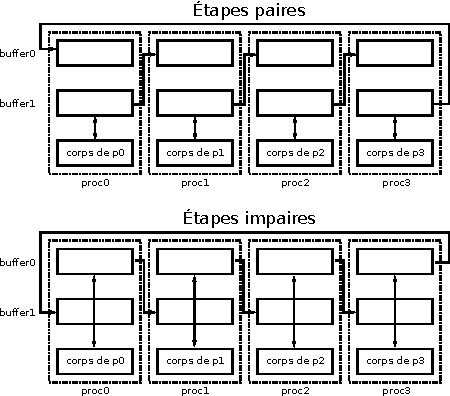
\includegraphics[width=0.65\linewidth]{schemas/anneau_avec_buffering.pdf}
		\caption{Anneau de communication pour 4 processus MPI avec \textit{double buffering}}
		\label{fig:anneauDB}
	\end{figure}
	\begin{solution}
		Le problème de l'implémentation précédente c'est que l'on ne peut pas envoyer/recevoir des corps tant que les calculs ne sont pas terminés sinon on risque d'écraser les corps en cours de traitement.
		Le \textit{double buffering} permet d'éviter ce problème en utilisant deux \textit{buffers} MPI au lieu d'un seul.
		Il est ainsi possible d'envoyer des corps à un processus même si ce dernier n'a pas terminé ses traitements.
		Il faudra aussi penser à inverser les \textit{buffers} à chaque étape (au sein d'une même itération) pour que cela fonctionne.
	\end{solution}
\end{questions}


\end{document}
